\pgfmathsetseed{2}
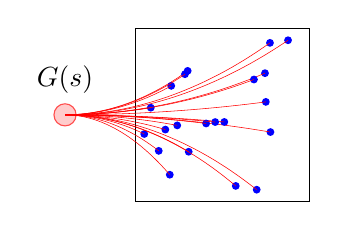
\begin{tikzpicture}
\draw (-1.1,-1.1) rectangle (1.1,1.1);
\node (seed) at (-2,0) [draw=red!70,fill=red!20, inner sep=1pt, minimum width=8pt, circle, label=above:$G(s)$] {};

\foreach \i in {0,1,...,20}
    {
    \node (p\i) at (rand,rand) [inner sep=1pt, minimum width=2pt, circle, fill=blue] {};
    \draw[-,very thin,red] (seed) parabola (p\i);
    }

%\node at (2,0) [draw=red!70,fill=blue!20, inner sep=1pt, minimum width=2, rectangle, label=above:$r$] {};

\end{tikzpicture}